\chapter{PLANTEAMIENTO DEL PROBLEMA}
\section{Descripción de la Realidad Problemática}

De acuerdo al análisis del crecimiento y expansión urbana del Centro Nacional de Planeamiento Estratégico (CEPLAN) del 2023, menciona que con respecto al censo 2017 del INEI, ha crecido las zonas urbanas a un 1.6\% en comparación al censo de 2007, lo que quiere decir que la población urbana ha crecido en aproximadamente 3 millones de habitantes (CEPLAN,2023). Este crecimiento de la urbanización también a traído consigo un aumento significativo a las acciones criminales que enfrenta Perú, y también en todo el mundo; como es el caso de California (Estados Unidos), ya que se revela que los crímenes violentos, robos y asaltos agravados ha aumentado en un 5.7\% en el año 2023 (PPIC, 2023). Esto refleja una gran preocupación de la seguridad ciudadana en la que enfrenta la población y las autoridades que buscan tomar medidas cruciales para proteger a los residentes de los entornos urbanos. 

Él índice de criminalidad en Lima representa un 70.9\%, que se sitúa en el puesto número 17, por debajo de ciudades de Latinoamérica como Caracas (Venezuela), San Pedro Sula (Honduras) y Río de Janeiro (Brasil) que también enfrentan varios desafíos para reducir las acciones delictivas y mejorar la seguridad ciudadana (Numbeo, 2023). A pesar de eso, el índice de representatividad de crímenes en Lima no resta importancia a la clara necesidad de encontrar alternativas efectivas que permita reducir dicho índice de criminalidad en otras áreas urbanas del Perú.%\medskip
\begin{figure}[h]
	\begin{center}
		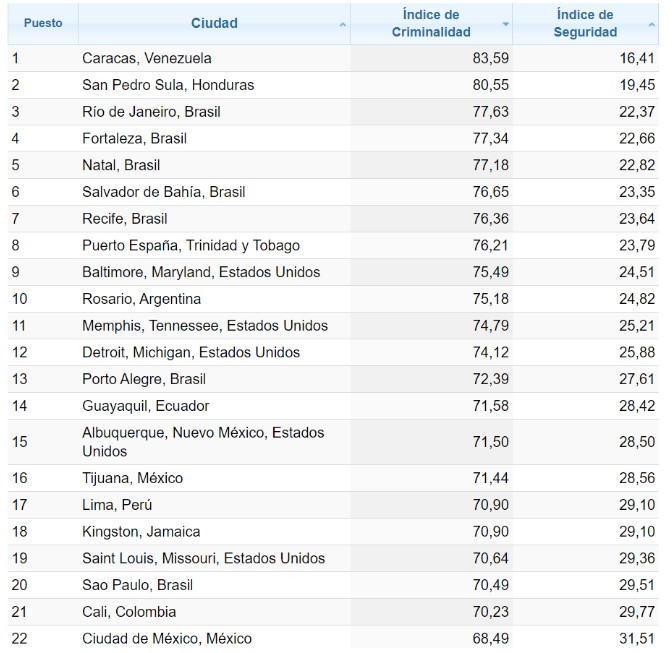
\includegraphics[width=0.65\textwidth]{1/figures/fig11.jpg}
		\caption{Índice de criminalidad de los países de América 2023}
		\label{1:fig}
	\end{center}
\end{figure}

Según datos recopilados en la plataforma de Statista entre Julio y diciembre del 2023, por cada 100 habitantes en las zonas urbanas de Perú, el 11.9\% de esta población ha sido víctimas por el robo de pertenencias personales, como dinero, carteras o celulares, siendo esta, la más representativa y la que refleja la parte vulnerable de los ciudadanos al no hacer frente a los robos que se cometen en las calles. Si se toma en cuenta el tipo de acto delictivo que puede atentar a la vida humana en las calles, se tiene que, el robo de vehículos representa un 2\%, mientras que el secuestro y extorsión el 0.2\%; que, si bien son menos frecuentes, representan una amenaza al bienestar y seguridad de los ciudadanos de las zonas urbanas (Statista Research Department, 2024). El último informe del Organismo Supervisor de Inversión Privada en Telecomunicaciones (Osiptel) de 2023, se registraron un total de 1,706,643 casos de robo de celulares en el año 2023, el cual el mayor número de robo ha sido los días lunes (Infobae, 2024). Asimismo, se informó que, entre el periodo de enero y mayo del año 2023, por cada hora, se roban en promedio, 200 celulares a nivel nacional (El Comercio, 2023). Estos resultados no solo representan una pérdida material y económica por parte de los afectados, genera desconfianza y preocupación sobre su seguridad personal y la posible vulneración en su privacidad de información que se contenía en el dispositivo del agraviado.
 %\medskip
\begin{figure}[h]
	\begin{center}
		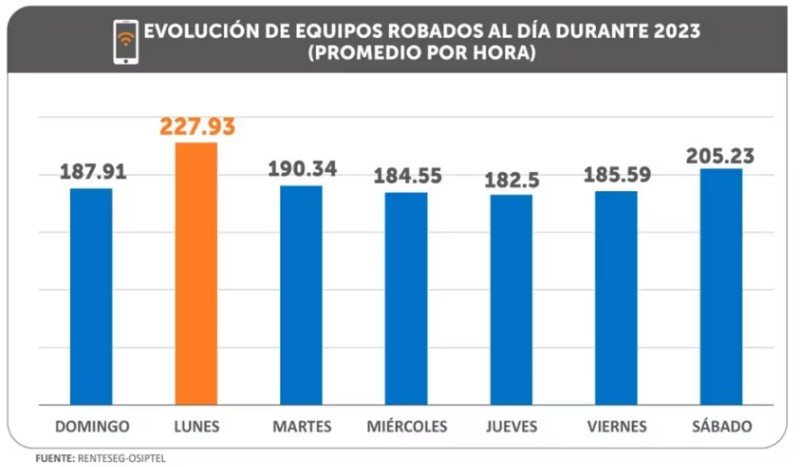
\includegraphics[width=0.65\textwidth]{1/figures/fig1.jpg}
		\caption{Días con más robos de celulares registrados en el 2023 Osiptel}
		\label{1:fig2}
	\end{center}
\end{figure}


Con lo que respecta al robo de vehículos, que también atenta a la vida y seguridad de la población de las zonas urbanas, según la Asociación Automotriz del Perú (APP) en el año 2023, la venta de vehículos ha representado un aumento del 2.4\% (181,000 autos vendidos) con respecto al año 2022 (AmChamnews, 2024). Este incremento en la venta de autos, también lleva consigo el aumento a los robos de vehículos, que es un problema que se está volviendo cada vez más persistente en Perú, ya que, según la Superintendencia Nacional de Registros Públicos, en promedio se roban 46 autos al día y que en el primer semestre del año 2022 se ha registrado un total de 9,758 autos robados en el Perú (Tracklink, 2023). 

Estas cifras demuestran la necesidad de desarrollar herramientas y/o estrategias que permitan mitigar los riesgos relacionados con los actos delictivos en entornos rurales, donde se destaca el robo de celulares y vehículos, que, a su vez, pueden estar relacionadas entre sí. Las aplicaciones móviles para ayudar al usuario a elegir rutas más cortas para llegar a su destino en el menor tiempo posible mediante un motor de crowdsourcing (recopilación de tráficos), son cada vez más comunes y fundamentales de utilizar; ya que, en 2022, más de 150 millones de personas utilizan Waze; mientras que Google maps ha sido instalada por más de 10 mil millones de usuarios (autocosmos, 2022). Sin embargo, estas herramientas de ayuda no tienen una funcionalidad que les permita detectar entre qué calles son seguras o no tomando en cuenta información o denuncias de delitos cometidos en esas zonas, ocasionando que los usuarios queden expuestos a situaciones peligrosas como el robo de su celular, de su auto o ambas. 



\section{Formulación del Problema}

Para lefecto \parencite{ot_marti2018manual}. 


Una vez elaborado el diagrama (véase Anexo 1), 

\subsection{Problema General}
\newcommand{\ProblemaGeneral}{
	¿Es posible utilizar algoritmos de aprendizaje profundo para detectar rutas seguras en las calles de los Ángeles? 
}
\ProblemaGeneral
\subsection{Problemas Espec\'{i}ficos}
\newcommand{\Pbone}{
¿Qué algoritmos de aprendizaje profundo son los más representativos de los antecedentes?
}
\newcommand{\Pbtwo}{
¿Qué alternativas de procesamiento de datos se deben aplicar a la base de datos para entrenar el modelo?
}
\newcommand{\Pbthree}{
¿Qué métricas propuestas en los antecedentes existen para ayudar en la eficiencia y eficacia del modelo propuesto?
}
\newcommand{\Pbfour}{
¿Qué impacto generaría los resultados en la confianza de los usuarios con respecto a la detección de rutas seguras con un margen de probabilidad de ocurrir un crimen?
}
\newcommand{\Pbfive}{
¿Qué impacto generaría los resultados en la confianza de los usuarios con respecto a la detección de rutas seguras con un margen de probabilidad de ocurrir un crimen?
}
\begin{itemize}
	\item \Pbone
	\item \Pbtwo
	\item \Pbthree
	\item \Pbfour
	\item \Pbfive
\end{itemize}

\section{Objetivos de la Investigación}
Para la formulación de los objetivos de la presente investigación se elaboró un «árbol de objetivos» (véase Anexo 2) 
\subsection{Objetivo General}
\newcommand{\ObjetivoGeneral}{
Evaluar algoritmos de aprendizaje profundo para detectar rutas seguras en las calles de los Ángeles.
}
\ObjetivoGeneral
\subsection{Objetivos Espec\'{i}ficos}
\newcommand{\Objone}{
Seleccionar los algoritmos de aprendizaje profundo más representativos de cada antecedente para la detección de rutas seguras.
}
\newcommand{\Objtwo}{
Seleccionar una alternativa de procesamiento de datos que permita entrenar un modelo de detección de rutas seguras.
}
\newcommand{\Objthree}{
Evalular la factibilidad del modelo con las métricas propuestas en los antecedentes para mejorar el tiempo de procesamiento con los menores recursos.
}
\newcommand{\Objfour}{
Evaluar el impacto del modelo de detección con respecto al margen de probabilidad de ocurrir un crimen.
}
\newcommand{\Objfive}{
Evaluar el impacto del modelo de detección con respecto al margen de probabilidad de ocurrir un crimen.
}


\begin{itemize}
	\item {\Objone}
	\item {\Objtwo}
	\item {\Objthree}
	\item {\Objfour}
	\item {\Objfive}
\end{itemize}

\section{Justificación de la Investigación}

\subsection{Teórica}
Esta investigación se realiza 

\subsection{Práctica}
Al culminar la investigación 

\subsection{Metodológica}. 

\section{Delimitación del Estudio}

\subsection{Espacial}
Para la presente investigación 

\subsection{Temporal}
Los datos que serán necesari. 

\subsection{Conceptual}
Esta investigación se 

\section{Hipótesis}

\subsection{Hipótesis General}
\newcommand{\HipotesisGeneral}{
El uso de técnicas de.
}
\HipotesisGeneral
\subsection{Hipótesis Específicas}
\newcommand{\Hone}{
	x
}
\newcommand{\Htwo}{
	y
}
\newcommand{\Hthree}{
	z	
}
\newcommand{\Hfour}{
	cv
}
\newcommand{\Hfive}{
	xws
}
\begin{itemize}
	\item \Hone
	\item \Htwo
	\item \Hthree
	\item \Hfour
	\item \Hfive
\end{itemize}

\subsection{Matriz de Consistencia}
A continuación se presenta la matriz de consistencia elaborada para la presente investigación (véase Anexo \ref{1:table}).

